\chapter{La Composition des services web}
%% TODO Introduire la notion de la composition et le plan du chapitre

%   % Dans le chapitres précédent, nous avons étudiés la description, la
% publication,  la découverte et la sélection de services Web
% élémentaire. L'autre concept fondamentale % est la composition des
% services web.
  
%   % The other fundamental concept is web service composition which
% sometimes overlaps or will merge with the process of WS
% discovery. WS composition is a mechanism of combining two or more
% basic services into a possibly complex service. It is used to solve
% complex problems by combining available basic services. It helps to
% accelerate rapid application development and facilitate service
% reuse from developer perspective % and from user perspective it
% increases complex service consumption. As mentioned earlier a
% composite service can be regarded as a combination of services invoked
% in % a predefined order and executed as a whole and that has more
% functionality than its components. WS composition is needed because
% finding a right service provider for the request is not an easy task
% on fast growing WWW sometimes it is even % impossible. Thus WS
% composition becomes necessary and inevitable. Composing WS from
% existing ones is an effective method to fill this gap.\cite{Omer2011}

%   Dans ce chapitre, nous présentons dans un premier temps les
% définitions et les types de composition de services Web présents dans
% la littérature. Ensuite, nous étudions .....
  
%   Enfin, un ensemble de travaux proposent des approches de la
% composition dynamiques des services web sémantiques.
  

\newpage

  \section{Définition et types de composition}
  \label{sec:defin-et-caract}

  Cette section a pour but d'exposer, d'une part, quelques définitions
  et objectifs de la composition des services Web proposées par la
  communauté, et d'autre part, les différents types et mécanismes de
  composition selon différents points de vue rencontrés dans la
  littérature.
  
  \subsection{Définitions}
    \label{sec:definitions}

    Martin \emph{et al.} \cite{martin2004owl} définissent
    la composition comme étant \emph{``le processus de sélection, de
      combinaison et d'exécution de services en vue
      d'accomplir un objectif donné''}.\\
  
    Selon S. Dustdar et W. Schreiner \cite{dustdar2005survey} :
    \emph{`` L'infrastructure de base des services Web suffit pour la
      mise en œuvre d'interactions simples entre un client et un
      service Web. Si la mise en œuvre d'une application métier
      implique l'invocation d'autres services web, il est nécessaire
      donc de combiner les fonctionnalités de plusieurs services
      web. Dans ce cas, nous parlons d'une composition de services
      Web''}.\\
    
    En d'autre terme, La composition de services Web désigne une
    opération qui consiste à construire de nouvelles applications ou
    services appelés \textbf{services composites} ou agrégats par
    l'assemblage ou l'agrégation de services existants nommés
    \textbf{services atomiques} ou
    élémentaires.\\

    Il existent différentes techniques de composition de services web
    développées par la littérature. ces techniques sont également
    classés en fonction de différents critères.

    Selon les travaux, les définitions des types de composition
    diffèrent d'une communauté de l'autre.

    Barros \emph{et al.} \cite{barros2006standards} classent la
    composition des services Web en trois catégories: orchestration,
    chorégraphie et comportementale.

    \cite{peltz2003web} de ça part distingue deux ...
    %% commment classifies la compositions ?
    %% \cite{fluegge2006challenges} Static vs dynamique.

    %% Les Procédés de coordination comme une vision (point de vue)
    %% d'une composition des services Web.

      \subsection{Procédés de coordination}
      \label{sec:proc-de-coord}

      %% Introduire la notion d'un procédé de coordination
      Selon Peltz \cite{peltz2003web}, Nous distinguons deux
      catégories de procédés de coordination utilisés pour décrire la
      composition de services dans un flot de processus métier. des
      procédés implémentant l'\emph{orchestration} de services et des
      procédés implémentant la \emph{chorégraphie} des services.

      % ces termes (\textit{orchestration} et \textit{chorégraphie})
      % décrivent deux aspects de création des processus métiers à
      % partir des services Web composites \cite{peltz2003web}.

      \begin{figure}[h]
    \centering
    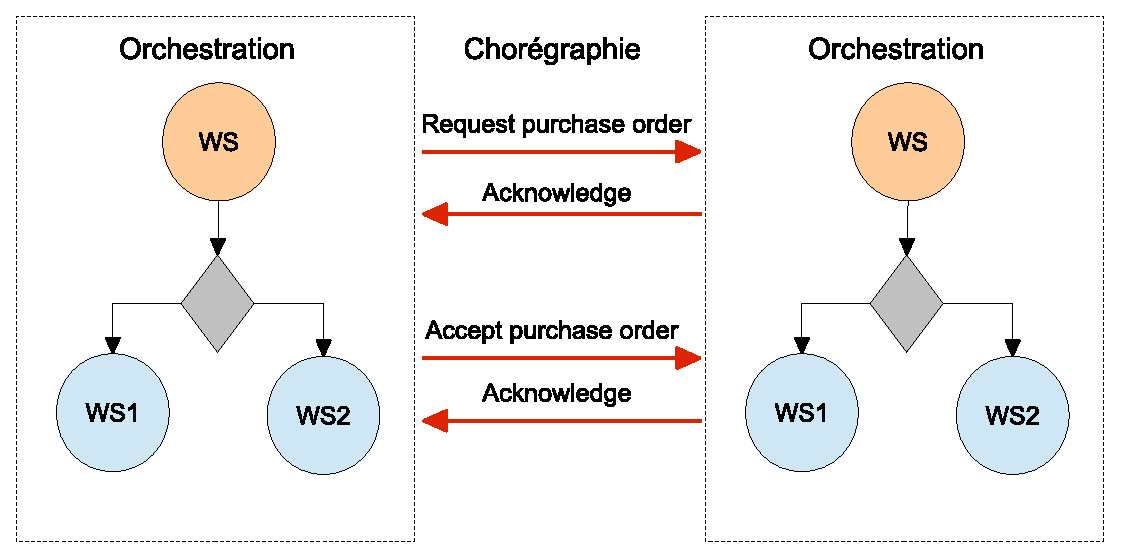
\includegraphics[width=1\textwidth]{figs/orchestration-vs-choregraphie.eps}
    \caption{Orchestration vs Chorégraphie selon Peltz
      \cite{peltz2003web}.}
    \label{fig:orchestration-vs-choregraphie}
\end{figure}

      \textbf{Un procédé} est représenté par un graphe orienté
      d'activités ou un flot de contrôle qui donne l'ordre d'exécution
      des activités et la logique de coordination des services. Chaque
      activité représente une fonctionnalité réalisée concrètement par
      un service \cite{chollet2009orchestration}. La figure
      \ref{fig:orchestration-vs-choregraphie} illustre ces deux
      approches en conjonction.
      % a figure orchestration vs chorégraphie

      % It should be noted that these models are not used exclusively:
      % one approach can implement more than one models at the same
      % time.\cite{baryannis2010} %% TODO: translate

        \subsubsection{Orchestration}
        \label{sec:orchestration}
        % Selon Sanlaville \cite{jamal2005environnement} : \emph{``
        %   L'orchestration des services Web permet de définir
        %   l'arranegement et l'enchaînement de ces services selon un
        %   canevas bien défini. Elle décrit la manière par laquelle les
        %   services peuvent interagir ensemble tout en incluant l'ordre
        %   d'exécution des différentes interactions''}.
        Barros \emph{et al.} \cite{barros2006standards} définissent
        l'orchestration comme un ensemble de processus exécutés dans
        un ordre prédéfini afin de répondre à un but
        \cite{lopez2008selection}. Ce type de composition se base sur
        un procédé métier exécutable permettant de décrire
        d'enchaînement et les interactions des différents services
        basiques collaborant dans une composition.

        L'orchestration offre \textbf{une vision centralisée} de
        contrôle, le procédé est toujours contrôlé par l'un des
        partenaires métiers. Ce dernier joue le rôle d'un chef
        d'orchestre qui se charge d'appeler les services de la
        composition suivant l'ordre d'exécution déjà défini par le
        processus métier.

        Le principe de l'orchestration est illustré
        par La figure \ref{fig:orchestration}.

        \begin{figure}[h]
    \centering
    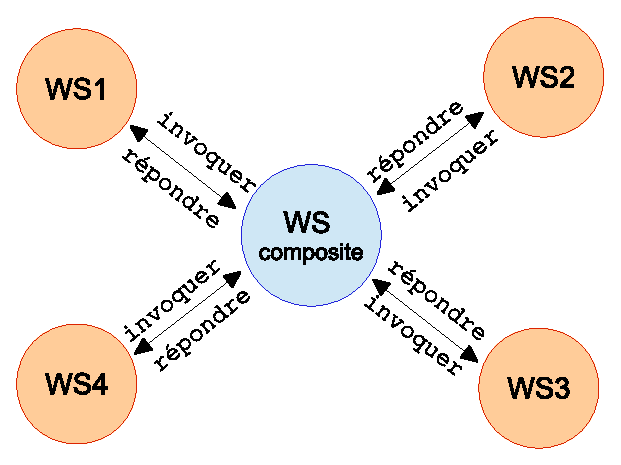
\includegraphics[width=0.6\textwidth]{figs/orchestration.eps}
    \caption{Principe de l’orchestration des services Web.}
    \label{fig:orchestration}
\end{figure}

        \subsubsection{Chorégraphie}
        \label{sec:choregraphie}
        % Selon Sanlaville \cite{jamal2005environnement} : \emph{`` La
        %   chorégraphie permet de tracer la séquence de messages
        %   échangés dans un contexte de composition de services
        %   Web. Elle est typiquement liée à la description de
        %   conversations existantes entre les services tout en
        %   impliquant plusieurs parties, incluant les clients, les
        %   fournisseurs et les partenaires''}.

        D'après Barros \emph{et al.} \cite{barros2006standards}, la
        chorégraphie permet de décrire la composition comme un moyen
        d'atteindre un but commun en utilisant un ensemble de services
        Web. La collaboration entre chaque service Web de la
        collection (faisant partie de la composition) est décrite par
        des flots de contrôle \cite{lopez2008selection}.

        La chorégraphie exprime une vue d'ensemble des services
        interagissant dans le cadre d'une composition de
        services. Selon Peltz \cite{peltz2003web}, la chorégraphie
        illustre les différants échanges de messages entre les
        participants. la chorégraphie offre \textbf{une vision
          décentralisée} et globale.

        Le principe de la chorégraphie est illustré par la figure
        \ref{fig:choregraphie}.

        \begin{figure}[h]
    \centering
    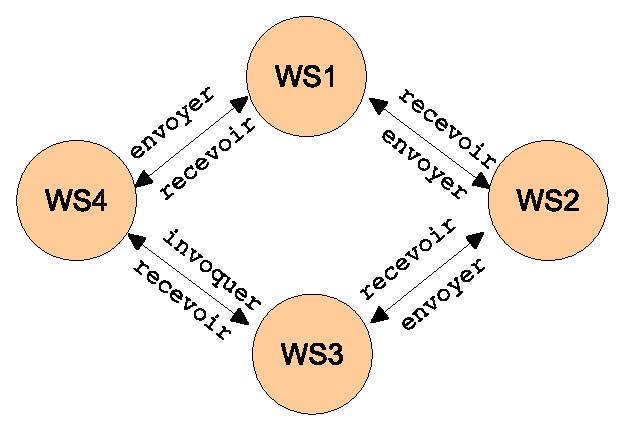
\includegraphics[width=0.6\textwidth]{figs/choregraphie.eps}
    \caption{Principe de la chorégraphie des services Web.}
    \label{fig:choregraphie}
\end{figure}


      \subsection{Types de composition}
      \label{sec:types-de-composition}
      Selon \cite{fluegge2006challenges}.

      La composition requiert la description et l'organisation de
      l'interaction entre les services. Elle nécessite la gestion de
      plusieurs aspects comme les échanges de données entre les
      services, les pannes ou erreurs éventuelles, le contexte
      d'interaction, le degré d'automatisation des tâches, etc. Dans
      la littérature, une variété de spécifications, de langages et
      d'approches formelles ont étudiés la composition.

      Dans la suite nous présentons les deux approches principales de
      description de la composition \emph{}n section
      \ref{sec:lang-de-comp}...
      \newpage

  \section{Languages de composition des services web}
  \label{sec:lang-de-comp}
  %% TODO: an introduction to the section
  Afin de supporter la composition de services, plusieurs langages de
  composition de services ont été proposés comme ...

  %% \cite{lopez2008selection}

    \subsection{BPEL}
    \label{sec:bpel}

    \acrshort{bpel} est une spécification du consortium OASIS
    \footnote{\url{https://www.oasis-open.org}}issue de la fusion des
    spécifications \acrshort{xlang} Microsoft
    \footnote{\url{http://www.microsoft.com}}et \acrshort{wsfl} d'IBM
    \footnote{\url{http://www.ibm.com}}, il hérite les
    caractéristiques d'un langage structuré en blocs de
    \textsc{XLANG}, ainsi que les caractéristiques d'un graphe direct
    de WSFL \cite{driss2011approche}.

    \textsc{BPEL} \textit{(appelé aussi \acrshort{bpel4ws} ou
      \acrshort{ws-bpel})} est le langauge d'orchestration le plus
    utilisé dans l'industrie permettant la coordination des
    interactions entre l'instance du service composite et ses
    partenaires sous forme d'un schéma \acrshort{xml} \textit{(le
      scriprt d'orchestration)}, il définit le processus,
    l'enchaînement et l'ordonnancement des actions qui seront
    exécutées par le moteur d'orchestration, agissant comme une
    machine virtuelle capable d'exécuter \textbf{le procédé métier}
    intéreptable de \textbf{coordination}
    \cite{chollet2009orchestration}.

    %% procédé abstraite vs exécutable
    %% les actions simples et composées, selon \cite{chollet2009orchestration}

    \subsection{WS-CDL}
    \label{WS-CDL}

    \subsection{OWL-S}
    \label{sec:owl-s}
    \cite{mcilraith2003bringing}

  \section{Compostion dynamique des services web}
  \label{sec:comp-dynam}
 
  \section{Conclusion}  
  \label{sec:conclusion}
 

%%% Local Variables: 
%%% mode: latex
%%% TeX-master: "../main"
%%% End: